\documentclass{standalone}

\usepackage{tikz}
\usepackage{circuitikz}

\tikzset{block/.style = {draw, fill=white, very thick, rectangle, minimum height=1cm, minimum width=2cm},
         lblock/.style={draw,fill=white,very thick, rectangle, minimum height=3cm, minimum width=1cm},
         sum/.style= {draw, fill=white, very thick, circle, node distance=0.5cm}}

         
\begin{document}
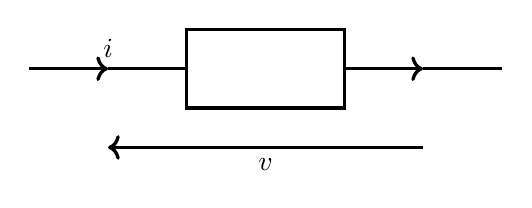
\begin{tikzpicture}[scale=2]
    \node[block](c)at(0,0){};
    \draw[->,very thick](-1.5,0)--(-1,0)node[above]{$i$};
    \draw[-,very thick](-1,0)--(c.180);
    \draw[->,very thick](c.0)--(1,0);
    \draw[-,very thick](1,0)--(1.5,0);
    \draw[->,very thick](1,-0.5)--(-1,-0.5)node[midway, below]{$v$};
\end{tikzpicture}
\end{document}